% SPDX-License-Identifier: CC-BY-4.0
%
% Copyright (c) 2023 Nelson Vieira
%
% @author Nelson Vieira <2080511@student.uma.pt>
% @license CC-BY-4.0 <https://creativecommons.org/licenses/by/4.0/legalcode.txt>
\documentclass[xcolor={svgnames},compress,aspectratio=169]{beamer}
\usetheme{Berlin}
\usecolortheme{dolphin}

\setbeamercolor*{structure}{bg=Azure,fg=MidnightBlue!50!black}

\setbeamercolor*{palette primary}{use=structure,fg=structure.bg,bg=structure.fg}
\setbeamercolor*{palette secondary}{use=structure,fg=structure.fg,bg=structure.bg}
\setbeamercolor*{palette tertiary}{use=structure,fg=structure.fg,bg=GhostWhite}
\setbeamercolor*{palette quaternary}{fg=white,bg=black}

\setbeamercolor{section in head/foot}{parent=palette primary} % Outer section of header/footer
\setbeamercolor{subsection in head/foot}{parent=palette secondary} % Inner section of header/footer

\setbeamercolor{titlelike}{parent=palette tertiary} % Main titles
\setbeamercolor{frametitle}{parent=palette tertiary,bg=GhostWhite!50}

\setbeamercolor{section in toc}{fg=darkgray,bg=Azure} % Table of contents sections
\setbeamercolor{subsection in toc}{fg=darkgray,bg=Azure} % Table of contents subsections
% \setbeamercolor{alerted text}{use=structure,fg=structure.fg!50!black!80!black}

% \setbeamertemplate{navigation symbols}{} % Hides navigation buttons at the bottom
% \setbeamertemplate{headline}{} % Hides navigation bar at the top

\setbeamercovered{transparent}

\setbeamertemplate{caption}[numbered]

% \usepackage{pgfpages}
% \pgfpagesuselayout{4 on 1}[a4paper,border shrink=5mm]

\usepackage[utf8]{inputenc}
\usepackage{adjustbox}
\usepackage{xcolor,colortbl}
\usepackage[all]{xy}
\usepackage{tikz}
\usetikzlibrary{mindmap,backgrounds}
\usepackage{graphicx}
\usepackage{multicol}
% Advanced table functions
\usepackage{tabularx,ragged2e}
\usepackage{booktabs}
% Listings extension
\usepackage{listings}
\usepackage{transparent}
\usepackage{amsmath,amssymb,amsfonts}
\usepackage[font=tiny]{caption}
\usepackage[font=tiny]{subcaption}
\usepackage{pgfplots}
\usepackage{pgf-pie}
\usepackage{tcolorbox}
\usepackage{svg}
\setsvg{inkscape = "C:/Program Files/Inkscape/bin/inkscape.exe"}
\svgsetup{inkscapepath=svgsubdir}
\def\myversion{0.9}

\title[Privacy in the Internet of Things: Fostering User Empowerment through Digital Literacy]{Master's Dissertation \\ {\normalsize Privacy in the Internet of Things: Fostering User Empowerment through Digital Literacy}}
% \subtitle{Empowering Users' Privacy Rights in the Internet of Things}
\author{\href{mailto:2080511@student.uma.pt}{Nelson Vieira}
\\ \and \textcolor{gray}{Orientation} \href{mailto:mary.barreto@staff.uma.pt}{Mary Barreto}
}
\institute[\href{https://www.uma.pt/}{University of Madeira}]{University of Madeira\\Faculty of Exact Sciences and Engineering}
\date{{\scriptsize Last Update: \today}}

\setbeameroption{hide notes}

\makeatletter
    \newenvironment{withoutheadline}{
        \setbeamertemplate{headline}[default]
        \def\beamer@entrycode{\vspace*{-\headheight}}
    }{}
\makeatother

\begin{document}

\begin{withoutheadline}
    \begin{frame}
        \centering
\includegraphics[width=90pt]{assets/images/uma_logo.png}
        \maketitle
    \end{frame}
\end{withoutheadline}

\begin{frame}{Table of Contents}
    % Use hideallsubsections for longer presentations
    % \tableofcontents[hideallsubsections]
    \begin{multicols}{2}
        \tableofcontents
    \end{multicols}
\end{frame}

\section{Introduction}

% Option [fragile] needed for lstlisting
\begin{frame}[fragile]
    \begin{multicols}{2}
        \centering
        {\footnotesize What is privacy?}
        \begin{figure}
            \centering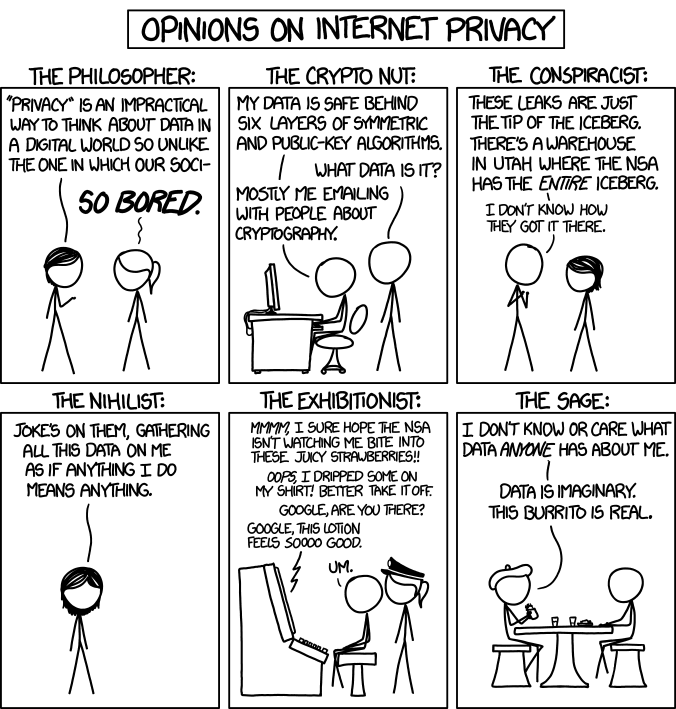
\includegraphics[width=155pt]{assets/images/privacy_opinions.png}\\
            \textcolor{gray}{{\tiny \textcopyright \href{https://xkcd.com/1269/}{Randall Munroe}, \href{https://creativecommons.org/licenses/by-nc/2.5/}{CC BY-NC 2.5 License}}}
        \end{figure}

        \columnbreak
        \vspace*{\fill}
\begin{lstlisting}[language=sh,escapechar=\%]
    diff privacy.c
    %\big\uparrow%     %\textcolor{blue}{@@ -42,1 +42,1 @@}%
    42 %\textcolor{red}{- Privacy}%
    42 %\textcolor{green!60!black!80}{+ Security}%
    %\big\downarrow%     ...
\end{lstlisting}
        \vspace*{\fill}
    \end{multicols}
\end{frame}

\note{
    There is some contention on the definition of privacy. Most literature assumes
    that privacy is equal to security or that it is only a part of it, as such
    by creating better security systems they assume to alse solve privacy problems.
    This work takes privacy on its own and goes out looking for challenges and solutions
    to solve privacy issues on IoT systems.
}

\begin{frame}{Introduction}
    Internet of Things (IoT) devices are everywhere. These devices
    create new ways of collecting and process personal data from users and
    non-users. Most end users are not even aware or have little control over
    the information that is being collected by these systems.

    This work takes an holistic approach to this problem by doing:
    \begin{itemize}
        \item<1-> Systematic literature review;
        \item<2-> A survey;
        \item<3-> A mobile application.
    \end{itemize}
\end{frame}

\note{
    This work tackles privacy literacy in IoT systems. An holistic approach was taken
    and consisted in doing a systematic literature review, a survey and a mobile application.
}

\section{State of the Art}

\begin{frame}
    \begin{figure}
        \centering
        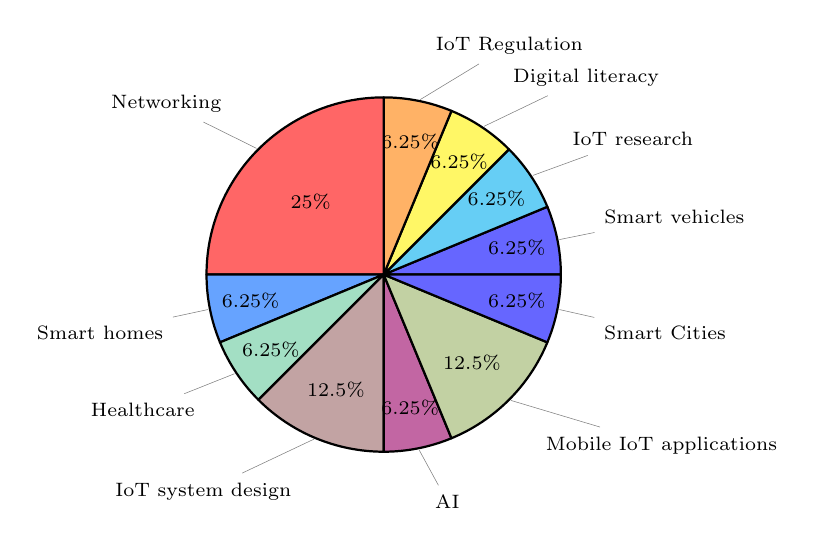
\begin{tikzpicture}
            \pie[text=pin,scale=0.75,font=\scriptsize]{6.25/Smart vehicles,
                6.25/IoT research,
                6.25/Digital literacy,
                6.25/IoT Regulation,
                25/Networking,
                6.25/Smart homes,
                6.25/Healthcare,
                12.5/IoT system design,
                6.25/AI,
                12.5/Mobile IoT applications,
                6.25/Smart Cities}
        \end{tikzpicture}
        \caption{Distribution of literature per IoT domain. (Chapter 6.1, p.67)}
        \label{fig:literature_domain}
    \end{figure}
\end{frame}

\note{
    + Blockchain
    + AI
    +/- Framework
    - Privacy notices

    Most literature works are on blockchain and AI solutions,
    followed by design or security frameworks and very few focus on privacy notices or legislation.
    Even fewer on privacy literacy.
}

\begin{frame}{State of the Art}
    \vspace*{\fill}
    There are two main ways to provide privacy in IoT systems:
    \vspace*{\fill}
    \begin{itemize}
        \item[$\bullet$]<1->
        Through security \cite{zhao2020local, zhang2017privacy, AliIoT, SunSecure};
        \item[$\bullet$]<2->
        Privacy notices \cite{FengDesign, DasPersonalized};
    \end{itemize}
    \vspace*{\fill}
    Legislation or a framework/architecture mainly fall into one these two categories.
    \vspace*{\fill}
\end{frame}

\note{
    abordagens
    Most literature approaches fall under privacy through security.
    Very few approach privacy as a unique concept with its own characteristics.
    Privacy literacy is barely taken on.
}

\section{Methodology}

\subsection{Survey}

\begin{frame}[shrink]{Survey}
    \begin{multicols}{2}
        86 Questions
        \begin{itemize}
            \item General knowledge and attitudes towards privacy
            \item Disposition for sharing personal information
            \item Privacy concerns
            \item Current online habits and practices
            \item Profile identification
            \item Knowledge and habits regarding the Internet of Things
            \item Demographic data
        \end{itemize}

        \columnbreak
        \vspace*{\fill}
        \begin{figure}
            \centering
            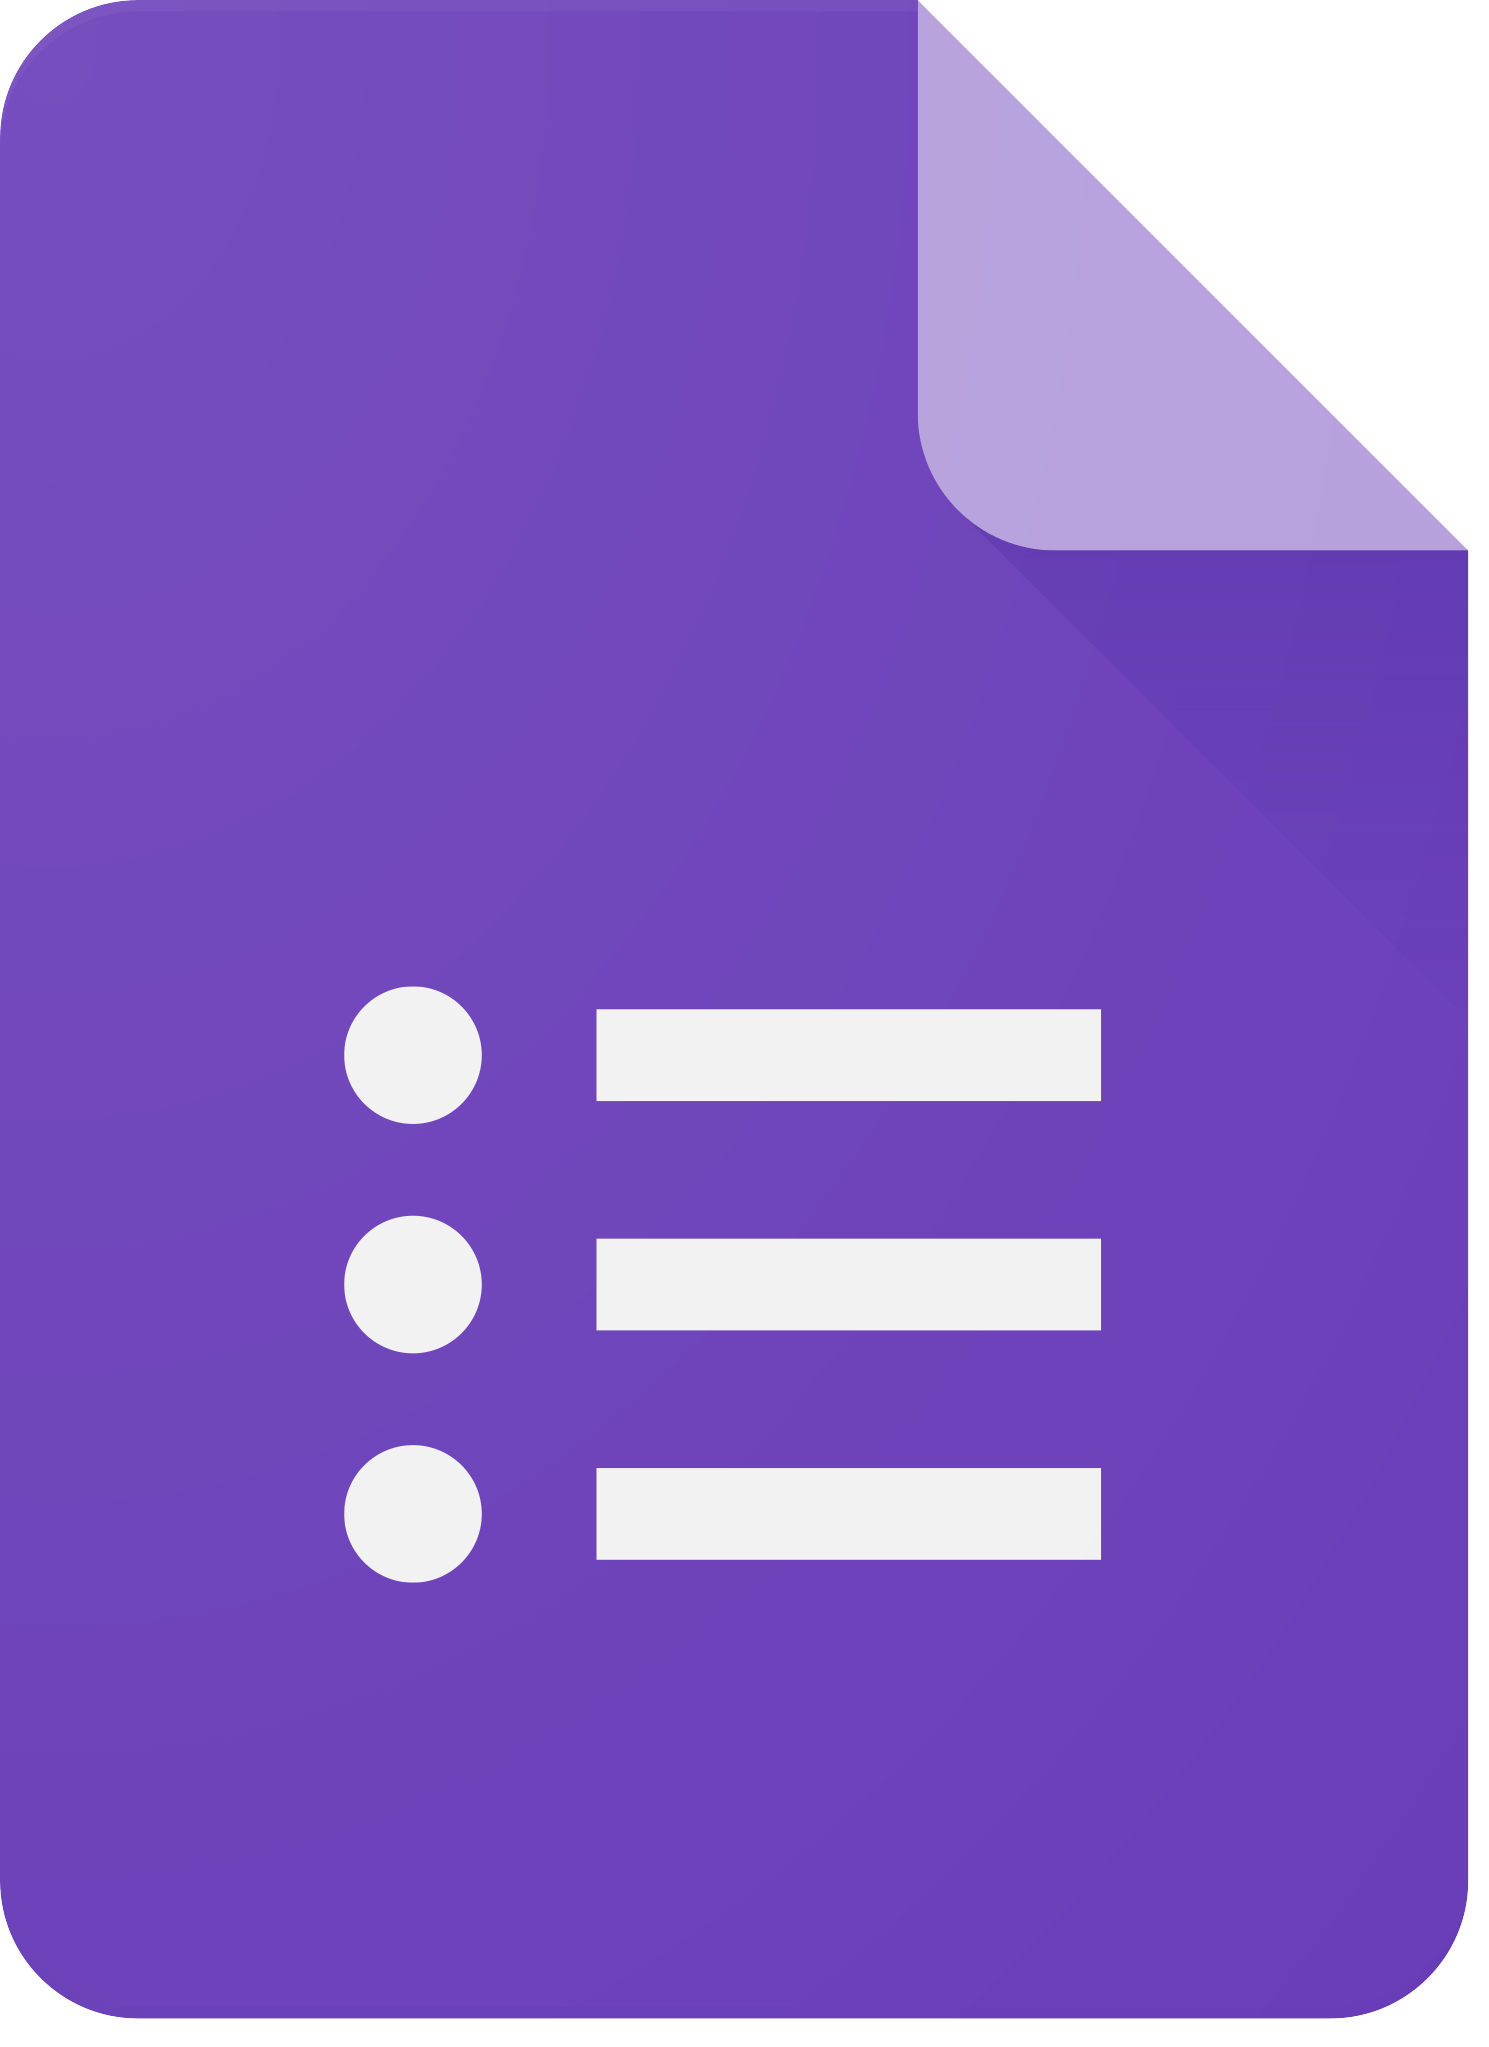
\includegraphics[width=45pt]{assets/images/forms.png}
            % \caption{Google Forms}
        \end{figure}
        \vspace*{\fill}
    \end{multicols}
\end{frame}

\note{
    Survey with varied questions from general privacy concerns to online habits and IoT literacy.
    86 questions under 7 main topics of interest from privacy attitudes, concerns, online habits to IoT knowledge and usage.
}
\begin{frame}
    \begin{multicols}{2}
        \begin{figure}
            \adjustbox{minipage=1.3em,valign=t}{\subcaption{}\label{sfig:survey_privacy_importance}}%
            \begin{subfigure}[t]{0.45\textwidth}
                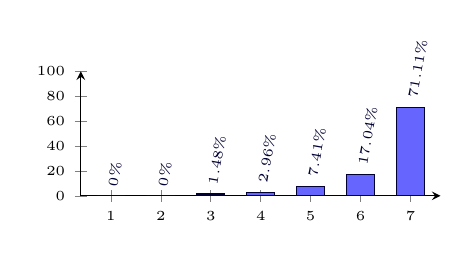
\begin{tikzpicture}
                    \begin{axis}[
                        width=175pt,
                        height=90pt,
                        ybar,
                        bar width=10pt,
                        ymin=0,
                        ymax=100,
                        xtick=data,
                        xtick style={font=\tiny},
                        ytick style={font=\tiny},
                        xtick style={font=\tiny},
                        ytick style={font=\tiny},
                        xticklabel style={font=\tiny},
                        yticklabel style={font=\tiny},
                        ylabel style = {font=\tiny},
                        xlabel style = {font=\tiny},
                        axis x line=bottom,
                        axis y line=left,
                        enlarge x limits=0.1,
                        nodes near coords={\pgfmathprintnumber\pgfplotspointmeta\%},
                        every node near coord/.append style={rotate=80, anchor=west, font=\tiny},
                        legend style={at={(0.5,-0.1)},anchor=north}
                    ]
                        \addplot[blue!20!black,fill=blue!60!white] coordinates {(1,0) (2,0) (3,1.48) (4,2.96) (5,7.41) (6,17.04) (7,71.11)};
                    \end{axis}
                \end{tikzpicture}
                % \caption{}
                % \label{fig:survey_privacy_importance}
            \end{subfigure}
            \adjustbox{minipage=1.3em,valign=t}{\subcaption{}\label{sfig:survey_it_terms}}%
            \begin{subfigure}[t]{0.45\textwidth}
                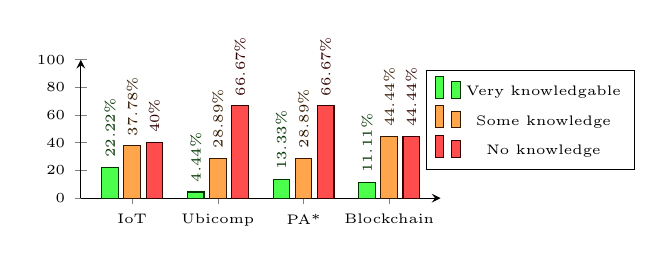
\begin{tikzpicture}
                    \begin{axis}[
                        width=175pt,
                        height=95pt,
                        symbolic x coords={IoT,Ubicomp,PA*,Blockchain},
                        ybar,
                        bar width=6pt,
                        ymin=0,
                        ymax=100,
                        xtick style={font=\tiny},
                        ytick style={font=\tiny},
                        xtick style={font=\tiny},
                        ytick style={font=\tiny},
                        xticklabel style={font=\tiny},
                        yticklabel style={font=\tiny},
                        ylabel style = {font=\tiny},
                        xlabel style = {font=\tiny},
                        axis x line=bottom,
                        axis y line=left,
                        enlarge x limits=0.2,
                        nodes near coords={\pgfmathprintnumber\pgfplotspointmeta\%},
                        every node near coord/.append style={rotate=90, anchor=west, font=\tiny},
                        legend style={at={(1.25,0.20)},anchor=south}
                    ]
                        \addplot[green!20!black,fill=green!70!white] coordinates {(IoT,22.22) (Ubicomp,4.44) (PA*,13.33) (Blockchain,11.11)};
                        \addlegendentry{{\tiny Very knowledgable}}
                        \addplot[orange!20!black,fill=orange!70!white] coordinates {(IoT,37.78) (Ubicomp,28.89) (PA*,28.89) (Blockchain,44.44)};
                        \addlegendentry{{\tiny Some knowledge}}
                        \addplot[red!20!black,fill=red!70!white] coordinates {(IoT,40) (Ubicomp,66.67) (PA*,66.67) (Blockchain,44.44)};
                        \addlegendentry{{\tiny No knowledge}}
                    \end{axis}
                \end{tikzpicture}
                % \caption{}
                % \label{fig:survey_it_terms}
            \end{subfigure}
            \caption{{\tiny Participant responses regarding: (a) participants' privacy importance perception and (b) general IT knowledge. (Chapter 5.1, p.49/51)}}
            \label{fig:survey_responses_privacy_importance_it_terms}
        \end{figure}

        \columnbreak
        % \hspace{0.2\linewidth}
        \begin{itemize}
            \item[$\bullet$]
            High regard for privacy, with some caveats;
            \item[$\bullet$]
            Some difficulty understating digital privacy;
            % \item[$\bullet$]
            % Different attitudes with different systems;
            \item[$\bullet$]
            Low literacy of technical jargon;
        \end{itemize}
        \vspace{2cm}
        \begin{flushright}
            {\tiny *PA - Privacy Assistant}
        \end{flushright}
    \end{multicols}
\end{frame}

\note{
    Majority of respondents found that privacy is very important.
    But lack knowledge about IoT and more esoteric IT or privacy topics.
}

\begin{frame}
    \begin{multicols}{2}
        \begin{figure}
            \begin{subfigure}[t]{0.45\textwidth}
                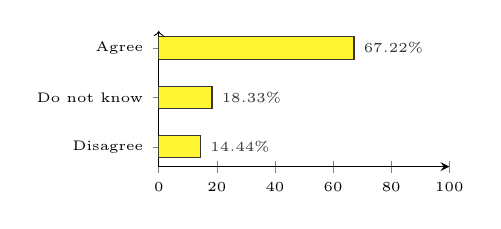
\begin{tikzpicture}
                    \begin{axis}[
                        width=150pt,
                        height=95pt,
                        xbar,
                        symbolic y coords={Disagree,Do not know,Agree},
                        bar width=8pt,
                        ytick=data,
                        axis x line=bottom,
                        axis y line=left,
                        xtick style={font=\tiny},
                        ytick style={font=\tiny},
                        xtick style={font=\tiny},
                        ytick style={font=\tiny},
                        xticklabel style={font=\tiny},
                        yticklabel style={font=\tiny},
                        ylabel style = {font=\tiny},
                        xlabel style = {font=\tiny},
                        xmin=0,
                        xmax=100,
                        enlarge y limits=0.2,
                        y axis line style={->,shorten >=1pt},
                        nodes near coords={\pgfmathprintnumber\pgfplotspointmeta\%},
                        every node near coord/.append style={font=\tiny},
                        legend style={at={(0.5,-0.1)},anchor=north, font=\tiny}
                    ]
                        \addplot[yellow!10!black,fill=yellow!80!white] coordinates {(14.44,Disagree) (18.33,Do not know) (67.22,Agree)};
                    \end{axis}
                \end{tikzpicture}
                {\tiny\caption{}}
                \label{fig:survey_privacy_notices}
            \end{subfigure}
            \begin{subfigure}[t]{0.45\textwidth}
                    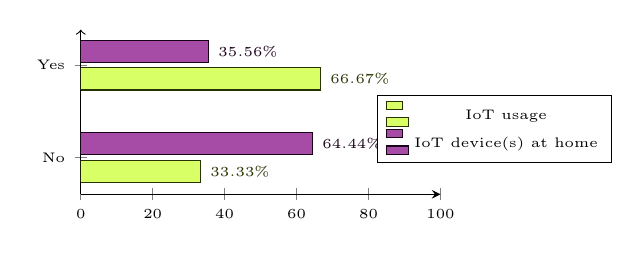
\begin{tikzpicture}
                        \begin{axis}[
                            width=175pt,
                            height=105pt,
                            xbar,
                            symbolic y coords={No,Yes},
                            bar width=8pt,
                            ytick=data,
                            xtick style={font=\tiny},
                            ytick style={font=\tiny},
                            xtick style={font=\tiny},
                            ytick style={font=\tiny},
                            xticklabel style={font=\tiny},
                            yticklabel style={font=\tiny},
                            ylabel style = {font=\tiny},
                            xlabel style = {font=\tiny},
                            axis x line=bottom,
                            axis y line=left,
                            xmin=0,
                            xmax=100,
                            enlarge y limits=0.4,
                            y axis line style={->,shorten >=0.5pt},
                            nodes near coords={\pgfmathprintnumber\pgfplotspointmeta\%},
                            every node near coord/.append style={font=\tiny},
                            legend style={at={(1.15,0.60)},anchor=north}
                        ]
                            \addplot[lime!20!black,fill=lime!60!white] coordinates {(33.33,No) (66.67,Yes)};
                            \addlegendentry{{\tiny IoT usage}}
                            \addplot[violet!20!black,fill=violet!70!white] coordinates {(64.44,No) (35.56,Yes)};
                            \addlegendentry{{\tiny IoT device(s) at home}}
                        \end{axis}
                    \end{tikzpicture}
                    {\tiny\caption{}}
                    \label{fig:internet_of_things_device_usage}
            \end{subfigure}
            \caption{Participant responses regarding: (a) unwillingness to read privacy notices and (b) IoT usage. (Chapter 5.1, p.55/58)}
            \label{fig:survey_responses_privacy_notices_iot_usage}
        \end{figure}

        \columnbreak
        \hspace*{\fill}
        \begin{itemize}
            \item[$\bullet$]
            Dismissal of privacy notices due to various factors;
            \item[$\bullet$]
            Some individuals use fake private data online;
            \item[$\bullet$]
            Some interaction with Internet of Things devices but low knowledge generally;
            \item[$\bullet$]
            Low grasp of IoT privacy;
        \end{itemize}
        \hspace*{\fill}
    \end{multicols}
\end{frame}

\note{
    Some notes here.
}

\subsection{Application}

\begin{frame}{Application}
    \begin{multicols}{2}
        What can the application do?
        \begin{itemize}
            \item Show the geolocation of the IoT devices;
            \item Information about the devices, like category, collection purpose, stored time, owner, etc.;
            \item Information about IoT privacy;
            \item Addition and editing of device's information.
        \end{itemize}

        \columnbreak
        \begin{figure}
            \centering
\includegraphics[width=120pt]{assets/images/flutter.png}
            % \caption{Flutter framework}
        \end{figure}
        \begin{figure}
            \centering
            \includesvg[width=140pt]{assets/images/firebase}
            % \caption{Firebase cloud backend}
        \end{figure}
    \end{multicols}
\end{frame}

\note{
    Some notes here.
}

{
\usebackgroundtemplate{{\transparent{0.1}\hspace*{0.2cm}
\includegraphics[keepaspectratio,width=7.5cm]{assets/images/icon.png}}}
\begin{frame}
    \centering
    \vspace*{\fill}
    {\Large Demonstration}
    \vspace*{\fill}
\end{frame}
}

\section{Conclusion and Future Work}

\subsection{Future Work}

\begin{frame}{Future Work}
    \begin{itemize}
        \item[$\bullet$]
        Privacy literacy in IoT systems;
        \item[$\bullet$]
        Application of privacy in the design/development of IoT systems;
        \item[$\bullet$]
        Interoperability standards;
        \item[$\bullet$]
        User-centric approaches to IoT privacy.
    \end{itemize}
\end{frame}

\note{
    Some notes here.
}

\subsection{Conclusion}

\begin{frame}{Conclusion}
    \begin{itemize}
        \item[$\bullet$]
        Standalone IoT privacy literature review;
        \item[$\bullet$]
        Tests from majority viewpoint of portuguese users;
        \item[$\bullet$]
        User testing reveals there is a large privacy knowledge gap;
        \item[$\bullet$]
        Application that aims to increase IoT privacy literacy.
    \end{itemize}
    % This work contributed to the overall body of research by compiling and reviewing
    % other works with the perspective of privacy as a distinct subject matter rather than
    % an extension of security, as many publications imply. The survey conducted
    % on the perception of individuals on privacy in IoT systems portrays the majority
    % viewpoint of portuguese people, since 60\% of participants were portuguese. Additionally,
    % a mobile application was developed and tested revealing that it performs as it was
    % initially designed and envisioned since it reaches its purpose on its own without having
    % to rely on additional platforms.
\end{frame}

\note{
    Some notes here.
}

\begin{frame}{Article submissions}
    \begin{itemize}
        \item[$\bullet$]
        Submission to EURASIP Journal on Information Security, under special issue: Multimedia
        Security and Privacy Protection in the Internet of Things (IoT) - \textit{Currently under review}
        \item[$\bullet$]
        Submission to e-Society 22nd International Conference 2024 - \textit{Currently under review}
    \end{itemize}
\end{frame}

\note{
    There are currently 2 article submissions based on the work conducted for this thesis,
    one submission for EURASIP Journal on Information Security,
    the other for e-Society 2024 conference in Porto
}

\begin{frame}
    \begin{center}
        {\large Thank you for your attention.}
    \end{center}
\end{frame}

\section*{References}

\begin{frame}[allowframebreaks]{References}
    \bibliographystyle{IEEEtran}
    {\footnotesize \bibliography{assets/references}}
\end{frame}

\end{document}
